\section{Limits on \mueee from Muon Decays}
In section \ref{sec:mu3e_experiment}, we saw how the production rate of $\mu^+$ at \mueee could be brought to the level of muon decays occuring at a rate $\order(10^9) \mu^+/s$.
The signal for the \mueee experiment, $\mu^+ \rightarrow e^+ e^+ e^-$, contains no missing energy as there are no neutrinos in the final state.
Since the experiment is looking at a muon beam, it can be expected that there will be many events that behave like a muon decay and have missing energy.
The SM has many avenues to produce such a signal with missing energy through muon decay, and we will go through the relevant backgrounds to our limits here.

\subsection{Backgrounds}
A strong irreducible background for the experiment is

\begin{equation}
    \mu^+ \rightarrow e^+ + \bar{\nu}_\mu + \nu_e + e^+ + e^-
\end{equation}

\noindent which comes with a branching ratio of $3.4 \times 10^{-5}$ \cite{Agashe:2014kda}. 
This is due to an internal conversion of muon to electron with a weak vertex, just like an ordinary muon decay.
To remove this background process, momentum conservation can be applied provided that the energy resolution is small enough.
For \mueee, a total energy resolution of $\sigma_E < 1\textrm{MeV}$ is sufficient for sensitivity of branching ratios down to $10^{-15}$ \cite{Blondel:2013ia}.
One such diagram for this process is shown in Fig.\ \ref{fig:mu_eeenunu_SM}.

\begin{figure}[h]
    \centering
    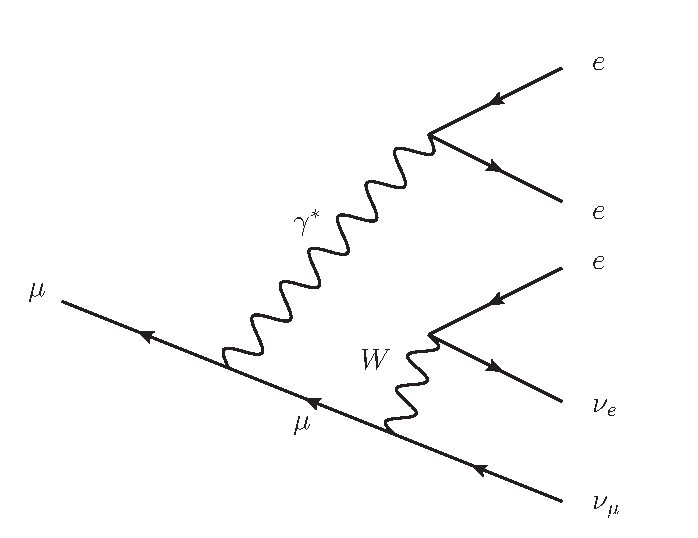
\includegraphics[width = 0.6\textwidth]{Figures/feynman_diagrams/mu_eeenunu_SM.eps}
    \caption{One Feynman diagram for the process $\mu^+ \rightarrow e^+ \bar{\nu}_\mu \nu_e e^+ e^-$. Here a virtual photon is emitted and decays to an $e^+ e^-$ pair. Note that the photon can be radiated off of any of the charged particles in the diagram before the $e^+ e^-$ decay. This background process can be suppressed by using momentum conservation with a high energy resolution.}
    \label{fig:mu_eeenunu_SM}
\end{figure}


Another source of background for the experiment is the radiative muon decay

\begin{equation}
    \mu^+ \rightarrow e^+ + \bar{\nu}_\mu + \nu_e + \gamma
\end{equation}

\noindent where the $\gamma$ radiates off of either the muon or electron.
This process comes with a branching ratio of $1.4 \times 10^{-2}$, given a photon energy larger than $10\textrm{MeV}$ \cite{Agashe:2014kda}.
The photon can then convert to an $e^+ e^-$ pair in the detector or target material, and mimic the irreducible background above.
Conversions outside of the target can be supressed if the vertex can be readily identified.
Within the target, this background appears as an accidental background with a regular muon decay.
